\chapter{Implementierung}
\label{chap:implementierung}

Dieses Kapitel dokumentiert die technische Implementierung der drei Hauptprojekte. Der Fokus liegt auf der detaillierten Beschreibung der Lösungsansätze, der aufgetretenen Herausforderungen und deren Bewältigung.

\section{TMC5160 Stepper-Motor-Driver}
\label{sec:tmc5160}

\subsection{Aufgabenstellung und technischer Hintergrund}

% TODO: Foto oder Schaltbild des Lötvorschub-Moduls einfügen?

Das erste Projekt konzentrierte sich auf die Mitentwicklung eines Lötvorschub-Moduls basierend auf dem TMC5160 Stepper-Motor-Controller von Trinamic. Das Modul wurde in C++ geschrieben und mittels C-Wrapper in die ATNC3-Firmware eingebunden.

Der Aufgabenbereich umfasste die Implementierung der Runtime-Berechnungen des Rampenprofils (Abbildung~\ref{fig:tmc_rampenprofil}).

\begin{figure}[h]
\centering
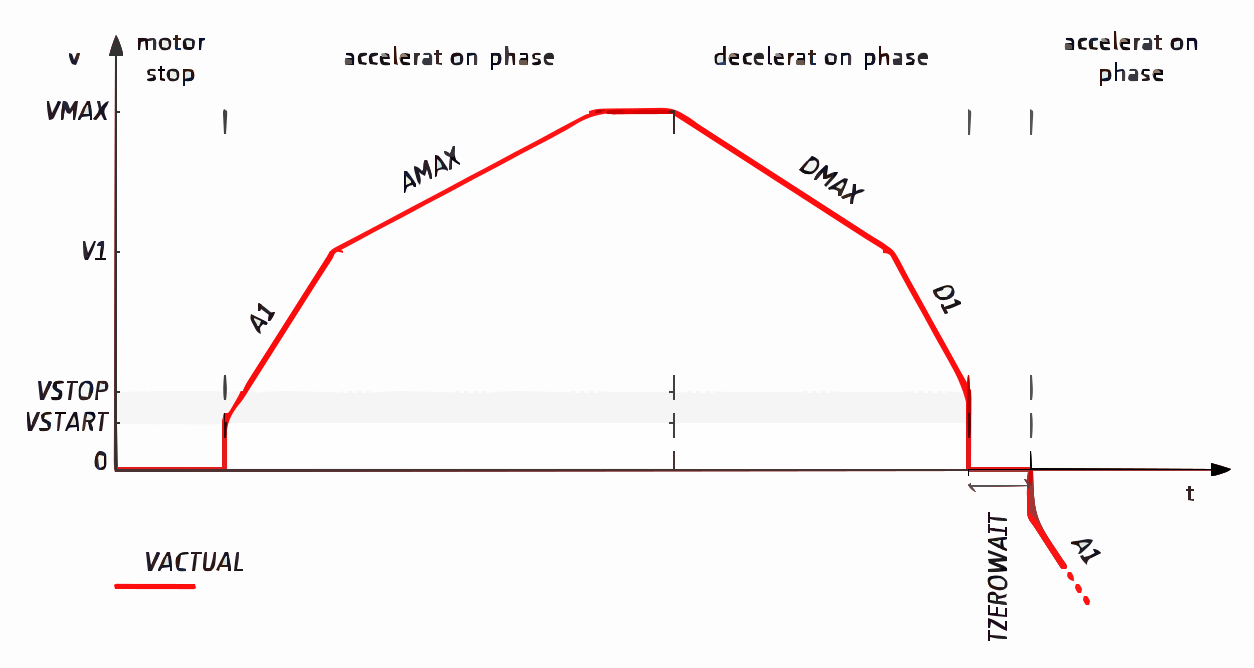
\includegraphics[scale=.6]{chapters/4_implementierung/graphics/tmc_ramp_profile.png}
\caption{TMC5160 Rampenprofil}
\label{fig:tmc_rampenprofil}
\end{figure}

\subsection{Mathematische Modellierung}

Das Rampenprofil wurde in fünf charakteristische Teilsektionen unterteilt (Abbildung~\ref{fig:tmc_rampenprofil_split}).

\begin{figure}[h]
\centering
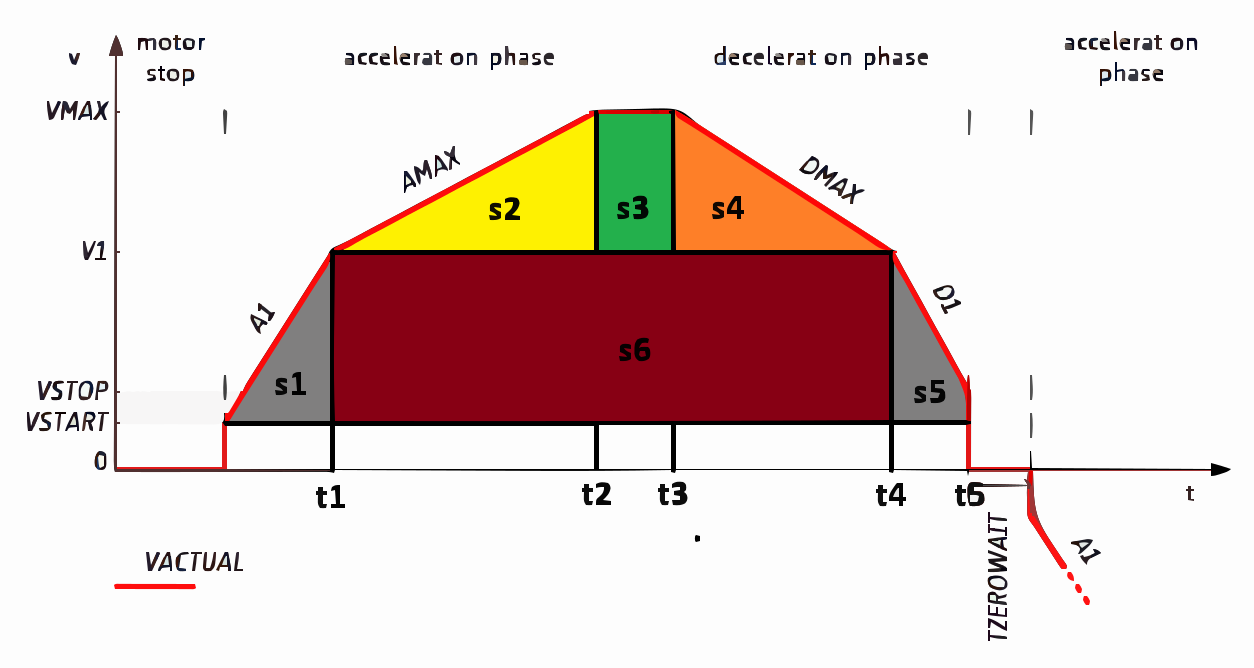
\includegraphics[scale=.6]{chapters/4_implementierung/graphics/tmc_ramp_profile_split.png}
\caption{Aufgeteiltes TMC5160 Rampenprofil mit Sektionen}
\label{fig:tmc_rampenprofil_split}
\end{figure}

\nlparagraph{Eingabeparameter}
Die benutzerdefinierten Eingabeparameter sind in Tabelle~\ref{tab:tmc5160_rampprofile_parameters} dargestellt.

\begin{table}[ht]
    \centering
    \begin{tabular}{c|c|l}
         Parameter & Einheit & Beschreibung \\ 
         \hline
         $V_{feed}$ & \unit{\frac{steps}{s}} & Vorschubgeschwindigkeit \\
         $V_1$ & \unit{\frac{steps}{s}} & Zwischengeschwindigkeit \\
         $t_{feed}$ & \unit{s} & Gesamtzeit \\
         $f_{accel}$ & \unit{\%} & Beschleunigungsfaktor \\
         $f_{decel}$ & \unit{\%} & Verzögerungsfaktor \\
    \end{tabular}
    \caption{Rampenprofil Eingabeparameter}
    \label{tab:tmc5160_rampprofile_parameters}
\end{table}

\nlparagraph{Randbedingungen}
Die Berechnungen erfolgen unter folgenden Randbedingungen:
\[V_{Stop} = V_{Start} = 0\]
\[t_{feed_{min}} = 0.1 < t_{feed} \]
\[S_{total} = V_{feed} \cdot t_{feed} = s_1 + s_2 + s_3 + s_4 + s_5\]

\nlparagraph{Berechnung von $V_{max}$}
Die maximale Geschwindigkeit wird wie folgt berechnet:
\[\mu_1 = 2 \cdot t_{feed_{min}} + \frac{(t_{feed} - 2 \cdot t_{feed_{min}}) \cdot (f_{accel} + f_{decel})}{2}\]
\[\mu_2 = (t_{feed} - 2 \cdot t_{feed_{min}}) \cdot (1 - \frac{f_{accel}}{2} - \frac{f_{decel}}{2})\]
\[V_{max} = \frac{V_{feed} \cdot t_{feed} - V_1 \cdot \mu_1}{\mu_2}\]

\nlparagraph{Rampenparameter}
Die Beschleunigungs- und Verzögerungswerte werden wie folgt modelliert:
\[A_1 = \frac{V_1}{t_1}, \quad A_{max} = \frac{V_{max} - V_1}{t_2}\]
\[D_1 = \frac{V_1}{-t_5}, \quad D_{max} = \frac{V_1 - V_{max}}{t_4}\]

\subsection{Programmatische Implementierung}

Die Implementierung erfolgte als Teil der \texttt{sf\_stepper}-Klasse. Die Funktion gliedert sich in mehrere Phasen:

\nlparagraph{Eingabevalidierung}
Zunächst erfolgt eine Validierung der Eingabeparameter zur Vermeidung ungültiger Berechnungen.
\lstinputlisting[caption=Eingabeparameter-Validierung, label={lst:input_validation}, language=C++]{chapters/4_implementierung/code/input_validation.c}

\nlparagraph{Berechnung}
Nach erfolgreicher Validierung werden die Einheiten konvertiert und $V_{max}$ berechnet.
\lstinputlisting[caption=Unit-Konversion und $V_{max}$-Berechnung, label={lst:vmax_calculation}, language=C++]{chapters/4_implementierung/code/vmax_calculation.c}

\nlparagraph{Konsistenzprüfung}
Abschließend erfolgt eine Plausibilitätsprüfung der Berechnungen mit definierten Toleranzen (zeitlich: 3ms, räumlich: 1 Fullstep $\approx$ 109µm).
\lstinputlisting[caption=Validierung der Berechnungen, label={lst:calculation_validation}, language=C++]{chapters/4_implementierung/code/calculation_validation.c}

\section{Hardware-Testing und Prototyping}
\label{sec:hardware_testing}

\subsection{Aufgabenstellung}

Zur Validierung des in Abschnitt~\ref{sec:tmc5160} beschriebenen TMC5160-basierten Lötvorschub-Moduls wurde ein Messsystem zur Erfassung von Bewegungsdaten benötigt. Ziel war es, die berechneten Rampenprofile mit den tatsächlichen Bewegungen des Motors zu vergleichen. Die Anforderungen waren:
\begin{itemize}
    \item Erfassung von Positionsdaten zur Verifikation der Rampenprofile
    \item Bidirektionale Messung (X/Y-Achse)
    \item Kostengünstige und zeitnahe Umsetzung (6 Tage)
\end{itemize}

Als Lösung wurde ein optischer Maussensor gewählt, der über einen Raspberry Pi Pico als USB-Host ausgelesen wird.

\subsection{Technische Realisierung}

\nlparagraph{USB-Host-Implementierung}
Der Raspberry Pi Pico wurde mittels TinyUSB-Stack und Pico PIO USB als USB-Host konfiguriert. Die PIO (Programmable I/O) des RP2040-Mikrocontrollers ermöglichte die USB-Kommunikation ohne dedizierte USB-Host-Hardware.

Die Implementierung umfasste:
\begin{itemize}
    \item Parsing des USB-HID-Protokolls
    \item Konfiguration der USB-Descriptors
    \item Interrupt-basierter Datentransfer
    \item Serielle Datenausgabe via UART
\end{itemize}

\nlparagraph{Mechanische Integration}

% TODO: Foto des Prototyps mit Maussensor und 3D-gedruckter Halterung einfügen?
% TODO: CAD-Screenshot der Halterung einfügen?

Für die Integration wurde eine Halterung mittels SolidWorks konstruiert und per FDM-3D-Druck gefertigt. Die Konstruktion berücksichtigte Sensor-Positionierung, mechanische Entkopplung und Fertigungsrestriktionen des FDM-Verfahrens.

\subsection{Evaluierung}

Die Implementierung der USB-Host-Funktionalität verlief erfolgreich. Bei der praktischen Evaluierung zur Verifikation der TMC5160-Rampenprofile zeigten sich jedoch kritische Einschränkungen des gewählten Sensorprinzips:

\begin{itemize}
    \item \textbf{Unzureichende Messgenauigkeit:} Die Abhängigkeit optischer Maussensoren von der Oberflächenbeschaffenheit führte zu inkonsistenten Messergebnissen (>5\% Fehler)
    \item \textbf{Sporadischer Tracking-Verlust:} Bei höheren Geschwindigkeiten oder inhomogenen Oberflächen gingen Messdaten verloren
    \item \textbf{Fehlende Reproduzierbarkeit:} Die Kalibrierungen zeigten hohe Streuung zwischen einzelnen Durchläufen
\end{itemize}

Durch diese Limitierungen waren die Testergebnisse für die Validierung der Lötvorschub-Rampenprofile unzuverlässig. Eine belastbare Aussage über die Korrektheit der TMC5160-Implementierung war mit diesem Messaufbau nicht möglich.

\subsection{Fazit}

Der Prototyp demonstrierte die technische Machbarkeit der USB-Host-Implementierung auf dem RP2040. Der gewählte Sensor-Typ erwies sich jedoch als ungeeignet für die geforderten Genauigkeitsanforderungen bei der Verifikation von Motorbewegungen.

Die gewonnenen Erkenntnisse führten zur Identifikation alternativer Ansätze für zukünftige Tests:
\begin{itemize}
    \item Lineare Encoder mit absoluter Positionserfassung
    \item Laser-basierte Distanzmesssysteme
    \item Inkrementalgeber mit höherer Auflösung
\end{itemize}

Trotz des negativen Evaluierungsergebnisses war die Entwicklungszeit von 6 Tagen akzeptabel, da der Rapid-Prototyping-Ansatz frühzeitig die technischen Grenzen des gewählten Sensorprinzips aufzeigte.

\section{W5500 Ethernet-Driver Integration}
\label{sec:w5500}

% TODO: Foto des W5500 Addon-Boards einfügen?
% TODO: Architekturdiagramm der Integration (SPI-Task, Buffer-Pool, etc.) erstellen?

Das Hauptprojekt der Praxisphase erstreckte sich über 3,5 Monate (08.08.2025 -- 24.11.2025) und umfasste die vollständige Integration eines W5500 Ethernet-Controllers in die ATNC3-Firmware. Zentrale Eigenentwicklung war dabei die Konvertierung des originalen WIZnet-Treibers von C zu C++ mit erweiterter Funktionalität.

\subsection{Projektphasen}

Das Projekt durchlief mehrere iterative Entwicklungsphasen:

\nlparagraph{Phase 1: Analyse und initiale Implementierung (Woche 1--3)}
\begin{itemize}
    \item Einarbeitung in Hardware-Dokumentation und W5500-Funktionsweise
    \item Entwicklung einer C++-basierten Testimplementierung
    \item Meilenstein: Funktionierende Grundkommunikation über Ethernet
\end{itemize}

\nlparagraph{Phase 2: Migration zu nativer C-Implementierung (Woche 4--6)}
\begin{itemize}
    \item Wechsel von C++ zu nativem C für Produktionsfirmware
    \item Wechsel von Evaluationsmodul zu eigenem Addon-Board
    \item Hardware-Registrierung im Bus-Device-Handler
    \item Meilenstein: Separat funktionierende C-Version
\end{itemize}

\nlparagraph{Phase 3: Firmware-Integration (Woche 7--9)}
\begin{itemize}
    \item Definition des genauen Projektumfangs
    \item Verlagerung SPI-abhängiger Funktionen in den SPI-Task
    \item Registrierung im Bus-Device-Handler
\end{itemize}

\nlparagraph{Phase 4: Interface-Entwicklung (Woche 10--12)}
\begin{itemize}
    \item Entwicklung des Ethernet-Interfaces
    \item Meilenstein: Driver integriert mit Interface für andere Module
\end{itemize}

\nlparagraph{Phase 5: Erweiterte Funktionalität (Woche 13--15)}
\begin{itemize}
    \item Implementierung statischer Buffer-Pools
    \item Implementierung asynchroner Read/Write-Funktionen
    \item Meilenstein: Produktionsreife Implementierung
\end{itemize}

\subsection{C++ Driver-Architektur}

Die C++-Testimplementierung bildete die Grundlage für das Verständnis des W5500 und diente als Referenz für die spätere C-Portierung. Der Driver wurde als objektorientierte Klassenhierarchie konzipiert, die Mehrfachvererbung nutzt.

\subsubsection{Klassenstruktur und Vererbung}

Die \texttt{W5500}-Klasse erbt von zwei Basisklassen mittels \texttt{protected} und \texttt{public} Vererbung:

\lstinputlisting[caption=W5500-Klassendeklaration mit Mehrfachvererbung, label={lst:w5500_class}, language=C++]{chapters/4_implementierung/code/w5500/w5500_class_declaration.cpp}

Diese Architektur ermöglicht:
\begin{itemize}
    \item \textbf{SPIDevice (protected):} Kapselung der SPI-Kommunikation, nicht direkt von außen zugreifbar
    \item \textbf{GPIO\_EXTI\_Handler (public):} Interrupt-Behandlung für eingehende Daten
\end{itemize}

\subsubsection{SPI-Abstraktionsschicht}

Die Basisklasse \texttt{SPIDevice} abstrahiert die hardwarenahe SPI-Kommunikation und verwaltet Chip-Select, DMA-Handles und Taktfrequenzen:

\lstinputlisting[caption=SPIDevice-Basisklasse, label={lst:spi_device}, language=C++]{chapters/4_implementierung/code/w5500/spi_device_class.cpp}

Die dynamische Baudrate-Konfiguration berechnet den optimalen Prescaler basierend auf der Peripheral-Clock:

\lstinputlisting[caption=SPI-Konfigurationsmethode mit Baudrate-Berechnung, label={lst:spi_configure}, language=C++]{chapters/4_implementierung/code/w5500/spi_configure.cpp}

\subsubsection{Interrupt-Handler-Pattern}

Für die Behandlung von GPIO-Interrupts wurde ein Handler-Pattern implementiert, das eine Zuordnung von GPIO-Pins zu Handler-Instanzen über eine statische Map ermöglicht:

\lstinputlisting[caption=GPIO-EXTI-Handler für Interrupt-Weiterleitung, label={lst:gpio_exti}, language=C++]{chapters/4_implementierung/code/w5500/gpio_exti_handler.cpp}

\subsection{Netzwerkkonfiguration}

\subsubsection{Konfigurationsstrukturen}

Die Netzwerkkonfiguration wird über typisierte Strukturen verwaltet:

\lstinputlisting[caption=Netzwerk-Konfigurationsstrukturen, label={lst:net_config}, language=C++]{chapters/4_implementierung/code/w5500/net_config.cpp}

\subsubsection{Initialisierung}

Der Konstruktor der W5500-Klasse initialisiert die Hardware vollständig:

\lstinputlisting[caption=W5500-Konstruktor mit Hardware-Initialisierung, label={lst:w5500_constructor}, language=C++]{chapters/4_implementierung/code/w5500/w5500_constructor.cpp}

Die SPI-Parameter werden über eine Konfigurationsstruktur übergeben:

\lstinputlisting[caption=SPI-Konfiguration für W5500 (25~MHz), label={lst:spi_config}, language=C++]{chapters/4_implementierung/code/w5500/spi_config.cpp}

\subsection{Socket-API}

Die Socket-API orientiert sich am Berkeley-Sockets-Interface, ist jedoch für Embedded-Systeme optimiert.

\subsubsection{Datenübertragung}

Die \texttt{send()}-Funktion implementiert nicht-blockierende TCP-Übertragung mit Zustandsverwaltung:

\lstinputlisting[caption=TCP-Send-Funktion mit Zustandsverwaltung, label={lst:send_func}, language=C++]{chapters/4_implementierung/code/w5500/send_function.cpp}

Bemerkenswert ist die Bit-Manipulation zur Verwaltung des Sendestatus pro Socket (\texttt{sock\_is\_sending}), die eine effiziente Zustandsspeicherung für alle 8 Sockets in einem einzigen Byte ermöglicht.

\subsubsection{Netzwerkkonfiguration zur Laufzeit}

Die Getter/Setter für Netzwerkparameter kapseln den Register-Zugriff:

\lstinputlisting[caption=Netzwerkkonfiguration-Funktionen, label={lst:netinfo_func}, language=C++]{chapters/4_implementierung/code/w5500/netinfo_functions.cpp}

\subsection{Register-Zugriff}

Der W5500 verfügt über Common Registers (netzwerkweit) und Socket-spezifische Register. Die Implementierung nutzt Makros zur Adressberechnung:

\lstinputlisting[caption=Register-Zugriffsmethoden, label={lst:register_access}, language=C++]{chapters/4_implementierung/code/w5500/register_access.cpp}

\subsection{Erweiterbare Kommando-Schnittstelle}

Für Debug- und Testzwecke wurde eine textbasierte Kommandoschnittstelle implementiert:

\lstinputlisting[caption=Erweiterbare Kommando-Tabelle, label={lst:command_table}, language=C++]{chapters/4_implementierung/code/w5500/command_table.cpp}

Die Kommando-Tabelle nutzt Funktionspointer auf Member-Methoden, was eine einfache Erweiterbarkeit ohne Änderung der Dispatcher-Logik ermöglicht.

\subsection{Technische Herausforderungen}

\subsubsection{Asynchrone SPI-Kommunikation}

Eine zentrale Herausforderung war die Implementierung asynchroner SPI-Kommunikation. In einem RTOS-System sind blockierende Aufrufe problematisch, da sie Task-Wechsel verhindern.

\nlparagraph{Problemstellung}
Die bestehende Firmware-Architektur sah eigene RTOS-Tasks für jeden SPI-Bus vor. Es fehlten jedoch:
\begin{itemize}
    \item Context-aware SPI-Funktionen
    \item Asynchrone Schnittstellen im W5500-Driver
    \item Callback-Mechanismen nach SPI-Transfer-Abschluss
\end{itemize}

\nlparagraph{Lösung}
Die implementierte Lösung nutzt freeRTOS-Mechanismen:
\begin{itemize}
    \item \textbf{Context-basierte Callbacks:} Jede SPI-Operation erhält Callback-Pointer und Context-Daten
    \item \textbf{Queue-basierte Verwaltung:} SPI-Requests werden in Queues eingereiht
    \item \textbf{Task-Synchronisation:} Semaphoren koordinieren den Bus-Zugriff
\end{itemize}

\subsubsection{Statisches Buffer-Management}

% TODO: Diagramm des Buffer-Pool-Konzepts erstellen (Allokation/Freigabe-Fluss)?

\nlparagraph{Problemstellung}
Dynamische Speicherallokation ist in Embedded Systems problematisch (siehe Kapitel~\ref{sec:speicherverwaltung}).

\nlparagraph{Lösung}
Entwicklung eines statisch allozierten Buffer-Pool-Systems:
\begin{itemize}
    \item Buffer werden zur Compile-Zeit allokiert
    \item Zur Laufzeit werden Buffer aus dem Pool angefordert
    \item Deterministische Allokationszeit (O(1))
    \item Thread-sichere Verwaltungsfunktionen
\end{itemize}

\subsubsection{Migration von C++ zu C}

Der Wechsel von der C++-Testimplementierung zu nativem C für die Produktionsfirmware erforderte fundamentale Designänderungen. Während die C++-Version Klassen und Vererbung nutzt, verwendet die C-Version Strukturen mit expliziten Handle-Pointern:

\begin{verbatim}
// C++ Version (Testimplementierung)
class W5500 {
    void sendPacket(uint8_t* data, size_t len);
private:
    uint8_t socket_state;
};

// C Version (Produktionsfirmware)
typedef struct {
    uint8_t socket_state;
} W5500_Handle_t;

void W5500_SendPacket(W5500_Handle_t* handle, 
                      uint8_t* data, size_t len);
\end{verbatim}

Objektorientierte Konzepte wurden durch Strukturen und Funktionen mit expliziten Pointern ersetzt. Kapselung wurde durch Funktionspräfixe (\texttt{W5500\_}) und \texttt{static}-Funktionen für interne Hilfsfunktionen erreicht.
